\problemname{Squawk Virus}

Oh no! Hackers are threatening to shut down Twitface, the premier social networking
site. By taking advantage of lax security protocols, nefarious cyber-bandits have
developed a virus that spreads from user to user, amplifying over time and eventually
bringing the network to its knees from massive congestion.  Normally users have to
manually send messages to one another (squawking), but these ne'er-do-wells have
figured out how to circumvent that rule, and have created squawks that spawn more
squawks without user intervention.  In particular, any time a user gets an infected
squawk, one minute later it broadcasts an infected squawk to all its neighbors in the
network (for purposes of this problem we assume that each neighbor gets the squawk
exactly 1 minute after the initial user is infected). If a user receives multiple
squawks at any point, the next minute it broadcasts that many squawks to all of its
neighbors.  For example, consider the following network:
\begin{center}
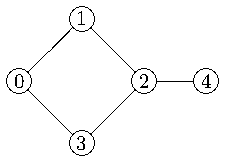
\includegraphics[width=0.3\textwidth]{graph}
\end{center}
If user $0$ is infected at time $t=0$, then at time $t=1$ users $1$ and $3$ get
$1$ squawk each, at time $t=2$ users $0$ and $2$ get $2$ squawks each, and at
time $t=3$, users $1$ and $3$ get $4$ squawks each and user $4$ gets $2$ squawks.

Given the layout of a social network and an initial infection site, you need to
determine how many squawks are made at some given time $t$.  In the above example
the number of squawks would be 2, 4 and 10 at times 1, 2 and 3, respectively.

\section*{Input}

The input will start with a line containing 4 integers $n$ $m$ $s$ $t$
indicating the number of users $(1\le n \leq 100)$, the number of links between
users $(0\le m \leq n(n-1)/2)$, the index of the initially infected user
$(s < n)$, and the number of minutes $(t < 10)$. Next will follow $m$ lines,
each consisting of two integers $x$ $y$, $(0 \leq x, y < n)$ indicating that
users $x$ and $y$ are connected. Connections are symmetric and no two
connections will be the same.
\newpage
\section*{Output}

Output the number of squawks sent at the specified time $t$.

